\chapter{Clustering} \label{chap:chap-2}

% if you want a short header you can use the following command
% \chapter[short-header-name]{chapter-title} \label{chap:chap-2}


% if you want to add the quote above the chapter heading then do the following:
% (for this case, you may have to change \ChapterTopSpace in the main file)
% \epigraphhead[0]{whole-above-epigraph-goes-here}


% add the citation for the chapter if it is a reprint


% add your chapter text here
\section{Introduction}
One of the many goals of the Matter Lab is the development of a self-driving laboratory. Cyclic voltammetry is an important part of the lab as it generates valuable mechanical information for redox-active chemical systems. 
\section{K-Means}
K-Means clustering is an unsupervised machine learning algorithm aimed to divide a set of data points into clusters such that the data points within each cluster are similar and different from the data points in other clusters \cite{MacQueen1967}. In this context, K represents the desired number of clusters. 
\begin{enumerate}
    \item Initially, K points are selected randomly as the cluster centroids
    \item Each data point is assigned to the closest mean, quantified by the Euclidean distance. 
    \item Each cluster centroid is updated to reflect the average of data points currently assigned to that cluster 
    \item This process is repeated for a specified number of iterations
\end{enumerate}

One of the questions that needs to be answered is the choice of K. This means finding a balance between the number of clusters represented by K and the average variance of the clusters while minimizing both. There is no approach that works better than all others in all cases. For this case, the elbow method is used by plotting the within-cluster sum of squares (WCSS) for a range of k and choosing the value k where adding more clusters does not significantly decrease the WCSS. 
\section{DBSCAN}
\section{t-Distributed Stochastic Neighbor Embedding}
t-Distributed Stochastic Neighbor Embedding (t-SNE) is a dimensionality reduction technique used for visualizing high-dimensional data in a low-dimensional space \cite{vanDerMaaten2008}. The similarity between two data points is represented by its euclidean distance. The first step of the algorithm is to create a probability distribution that represents the similarity between neighbors. For each data point, it is placed in the middle of the Gaussian curve and the rest of the data is placed along the curve. This is represented by the following equation where $j \neq i$ and $p_{i|i} = 1$:
\begin{align}
p_{j|i} = \frac{exp(-||x_i - x_j||^2 / 2\sigma_i^2)}{\sum_{k \neq i}exp(-||x_i - x_k||^2 / 2\sigma_i^2)}
\end{align}
"The similarity of datapoint $x_j$ to datapoint $x_i$ is the conditional probablity, $p_{j|i}$, that $x_i$ would pick $x_j$ if neighbors were picked in proportion to their probability density under a Gaussian centered at at $x_i$" \cite{vanDerMaaten2008}. The last variable that has not been discussed yet is sigma. This variable is not chosen directly, but rather by choosing a value for perplexity. Perplexity is defined as:
\begin{align}
Perp(p) \coloneq 2^{-\sum_x p(x)log_2(p(x))}
\end{align}
Perplexity represents the density of data and how many neighbors the central point should have with higher values relating to higher variance. After choosing the perplexity value, the corresponding sigma values are found using binary search. 
Next, the similarities between datapoints for low-dimensional representational will also need to be found to ensure that similar data are close together after projection. 
\section{UMAP}
\section{Curse of Dimensionality}
The curse of dimensionality refers to the phenomena that causes various challenges and complications when analyzing data in high-dimensional spaces. As the number of features in a dataset increases, the amount of data needed to generalize accurately grows exponentially. As the number of dimensions increases, the data becomes increasingly sparse. This makes tasks like clustering and classification more challenging. In higher dimensions, the difference between distances between data points start to become negligible, making measurements like Euclidean distance negligible. As such, algorithms that rely on distances measurements will experience a drop in performance. Furthermore, more dimensions will require more computational resources and time to process the data. 
\section{Ramer-Douglas-Peucker Algorithm}
The Ramer-Douglas–Peucker (RDP) algorithm is employed to reduce the number of points in a curve approximated by a series of points. It operates by conceptualizing a line between the initial and terminal points within a point set defining the curve. Subsequently, it identifies the point furthest from this line among the intermediary points. If this point, termed the "outlier point", and consequently all intervening points, lie within a specified distance 'epsilon' from the line, they are removed. Conversely, if the outlier point surpasses the epsilon threshold, the curve is segmented into two parts: from the initial point to the outlier point, inclusive and the outlier point and the remaining points. The algorithm is then recursively applied to both resulting segments, and the reduced forms of the curve are reassembled.
\section{Data Collection}
The data used was gathered through an automated electrochemistry experimentation that operates through through an iterative workflow \cite{PabloGarca2024}. The proposed workflow was used to synthesize and characterize 10 distinct metals and 10 distinct ligands resulting in 100 unique complexes. Each complex was synthesized using a metal/ligand concentration ratio of 1:7 to ensure complete complexation. The synthesis process employed 1.0 M NaCl in water as the electrolyte/solvent, and a buffer solution consisting of a 1:1 ratio of HOAc/NaOAc. Following synthesis, comprehensive characterizations were conducted using cyclic voltammetry (CV) and differential pulse voltammetry (DPV) techniques. This thorough investigation yielded a substantial database comprising 400 voltammetry datasets. Importantly, our workflow is adaptable, with the potential to encompass a broader range of parameters, including additional ligands, varying metal/ligand ratios, mixed ligands, different buffer pH levels, and reaction times. The accumulation of data points is ongoing, contributing to the continuous expansion and refinement of our understanding.
\section{Data Preparation}
With cyclic voltammetry data, there are many different variables that are unique to each experiment. Particularly, the experiment's scan rate affects the sampling frequency and resolution of data points collected over a given time interval. The length of data obtained changes with the scan rate. However, many data investigation techniques require the data to be the same length. Similarly, the potential limit at which the potential begins to return to its initial point will affect the overall shape of the cyclic voltammogram. To handle this, the following steps are used to prepare the data:
\begin{enumerate}
    \item Split experiment cycles into separate data points
    \item Normalize values to fit between [0, 1]
    \item Reduce points using the Ramer-Douglas-Peucker algorithm
    \item Duplicate datapoints until total length reaches the longest cycle's length
    \item Order datapoints based on angular position relative to the center
\end{enumerate}
Due to the curse of dimensionality, the RDP algorithm is used to reduce the number of dimensions. Since the RDP algorithm takes only a variable $\epsilon$, the final length after reduction will be different for each set of data. To ensure the data has the same length as the longest data after RDP reduction, datapoints are randomly selected and duplicated. Similarly, by ordering the data based on its angular position, the overall shape of the cyclic voltammogram is maintained.
\section{Results and Discussion}
To cluster the data using K-Means, a value of K will need to be selected. This is done using the elbow method. As seen in Figure \ref{elbow}, there are many valid values for K, and it is difficult to definitely say which value of K is best.
\begin{figure}[h!]
  \centering
    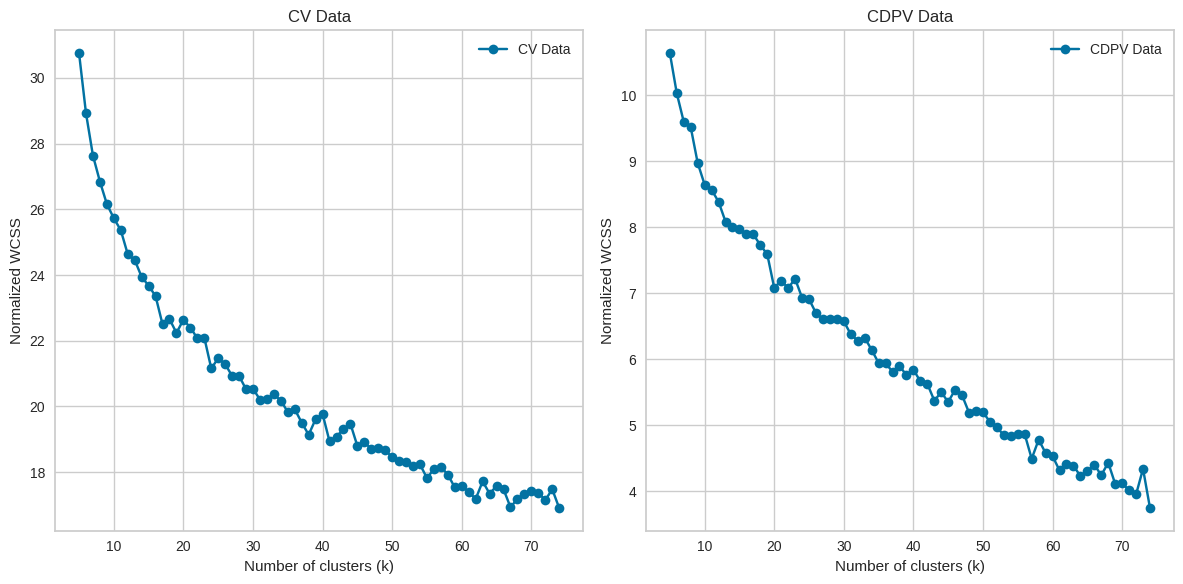
\includegraphics[width=1.0\textwidth]{figures/elbowmethod.png}
    \caption{K-Means Elbow Method}
    \label{elbow}
\end{figure}
To aid the decision-making process, the Silouhette method is used to analyze promising values. A cluster with a value of 1 means points are perfectly assigned in a cluster and clusters are easily distinguishable, 0 means clusters are overlapping, and -1 means points are assigned to the wrong cluster \cite{ROUSSEEUW198753}. The K value should be chosen based on which value produces the most clusters with Silhouette scores greater than the average score of the dataset, represented by the red-dotted line. Furthermore, there should not be wide fluctuations in the size of the clusters. The width of the clusters represents the number of data points belonging to the cluster. 
\begin{figure}[h!]
  \centering
    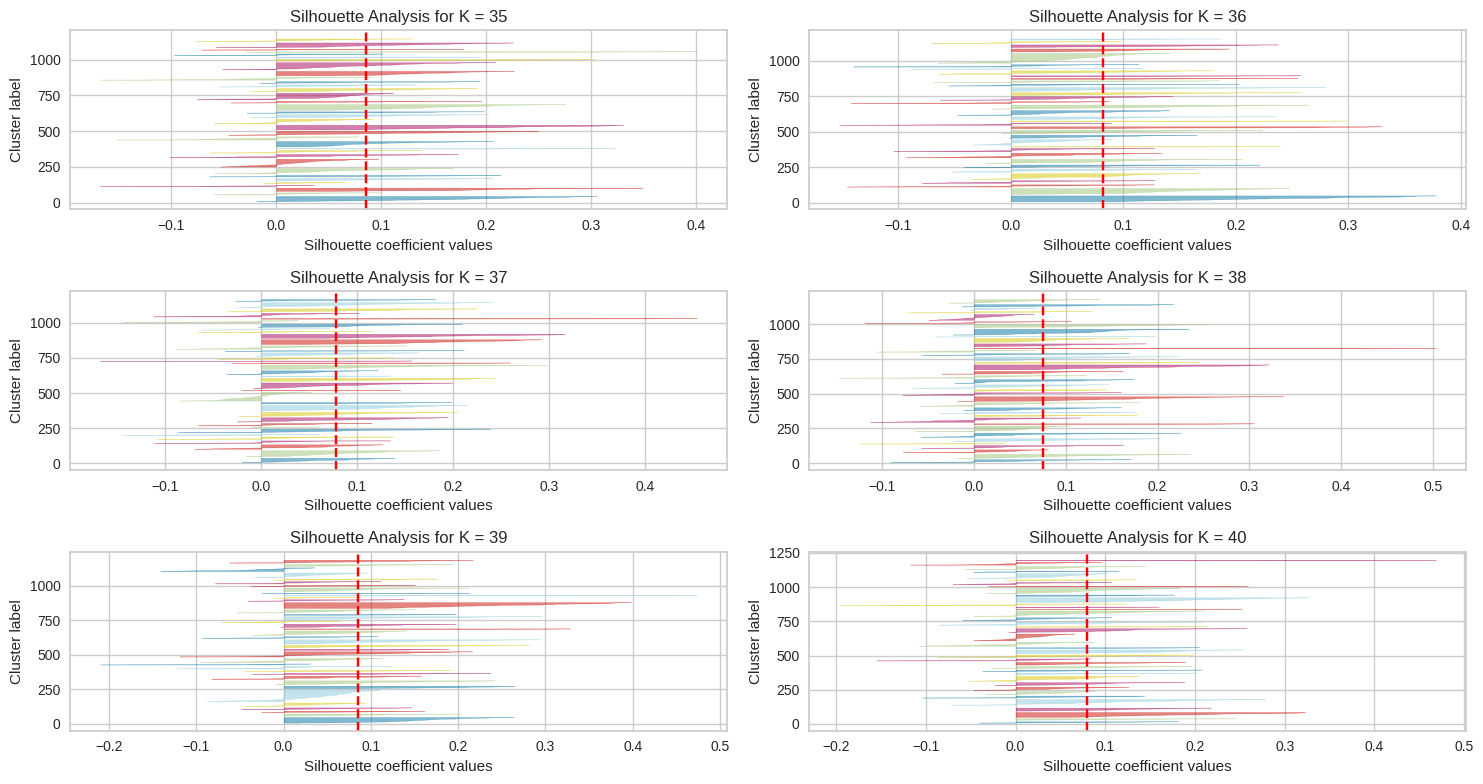
\includegraphics[width=1.0\textwidth]{figures/cv_silhouette.png}
    \caption{CV Silhouette Method}
    \label{cv_silhouette}
\end{figure}
In Figure \ref{cv_silhouette} showcasing the Silhouette method for CV, K = 38 results in the most clusters with a score above the dataset mean while also minimizing the number of clusters with a score below zero and minimizing the variance in the size of clusters. 
\begin{figure}[h!]
  \centering
    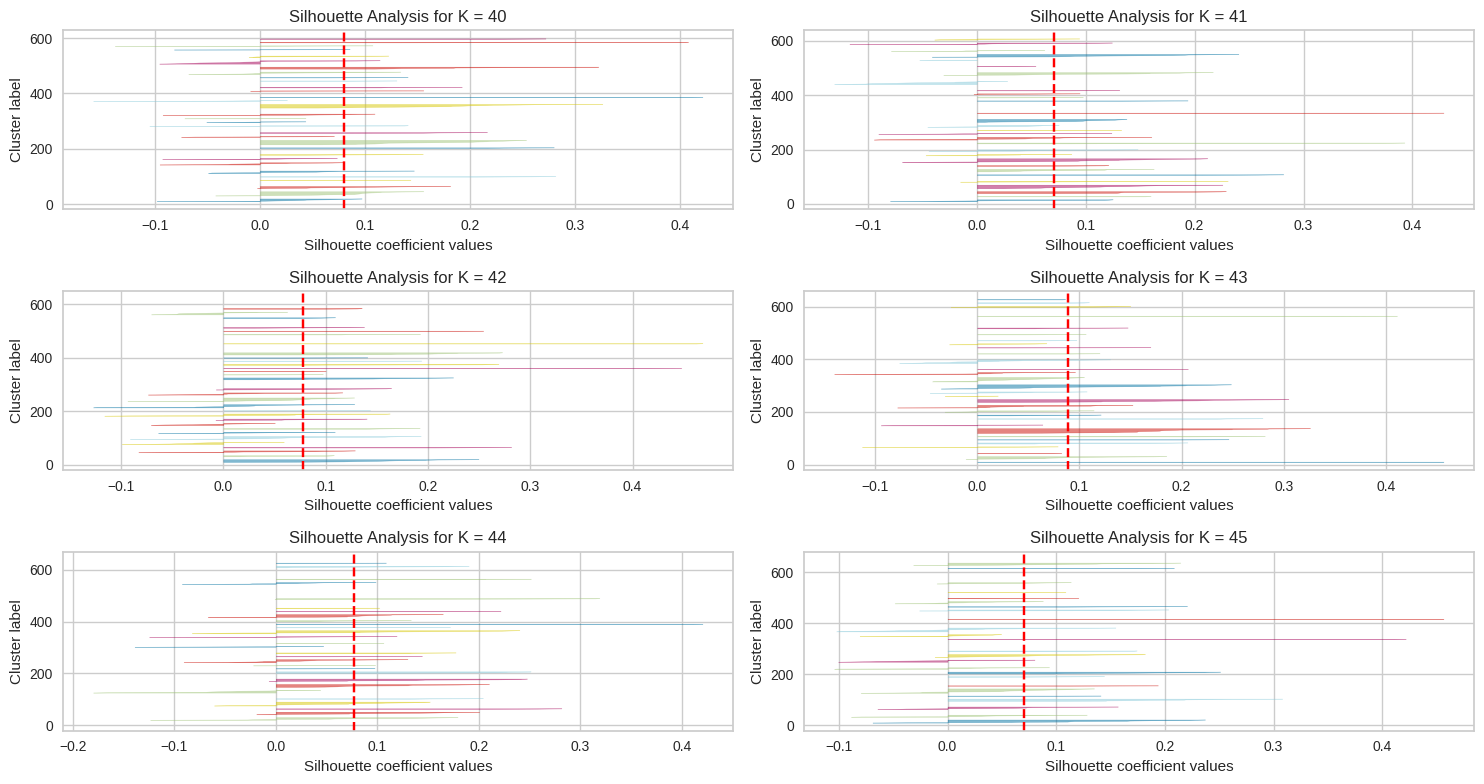
\includegraphics[width=1.0\textwidth]{figures/dpv_silhouette.png}
    \caption{DPV Silhouette Method}
    \label{dpv_silhouette}
\end{figure}
Similarly, in Figure \ref{dpv_silhouette} showcasing the Silhouette method for DPV, K = 42 results in the best quality of clusters. A subset of the cluster results is available in the appendix. Despite having 100 different combinations of metals and ligands, using a relatively small K value still shows promising results, as the datapoints within each cluster have similar overall shape. To further demonstrate the efficacy of the encoding and classification, t-SNE and UMAP projections are created to visualize the data in 2-D and show how the shapes, metals, and ligands are distributed. Interactive plots made with Bokeh are available.
As seen in the resulting figures \cref{cv-tsne, cv-umap, dpv-tsne, dpv-umap}, t-SNE emphasizes local structure and tends to agglomerate similar data points into tight clusters. As a result, t-SNE plots often show clearer separation between clusters but may not preserve the global structure as effectively. t-SNE primarily preserves local neighborhoods, which leads to tighter clusters of similar points. However, it may not always capture the global structure accurately, especially for complex datasets. t-SNE embeddings can vary significantly with different random initializations and parameter choices, making it less stable and potentially more sensitive to noise in the data. 
UMAP tends to focus more on preserving global structure and maintaining relative distance between clusters. Therefore, clusters in the UMAP plot are usually well separated and evenly distributed. UMAP tries to preserve local and global neighborhoods, resulting in more evenly spaced clusters and better representation of both local and global structures. UMAP embeddings are generally more stable across different runs and parameters settings compared to t-SNE.
\begin{figure}[h!]
  \centering
    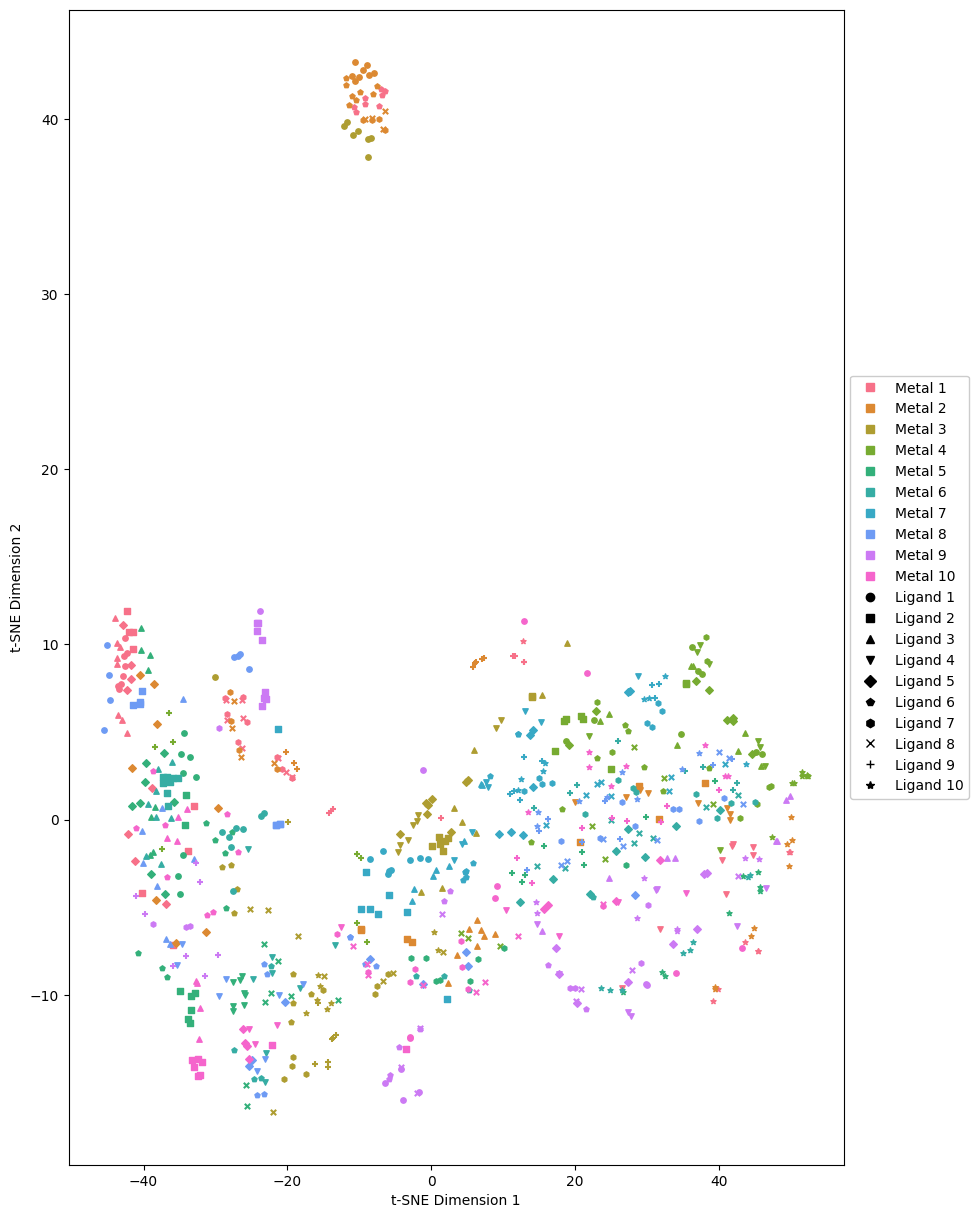
\includegraphics[width=1.0\textwidth]{figures/cv_tsne.png}
    \caption{Cyclic Voltammetry t-SNE Projection}
    \label{cv-tsne}
\end{figure}
\begin{figure}[h!]
  \centering
    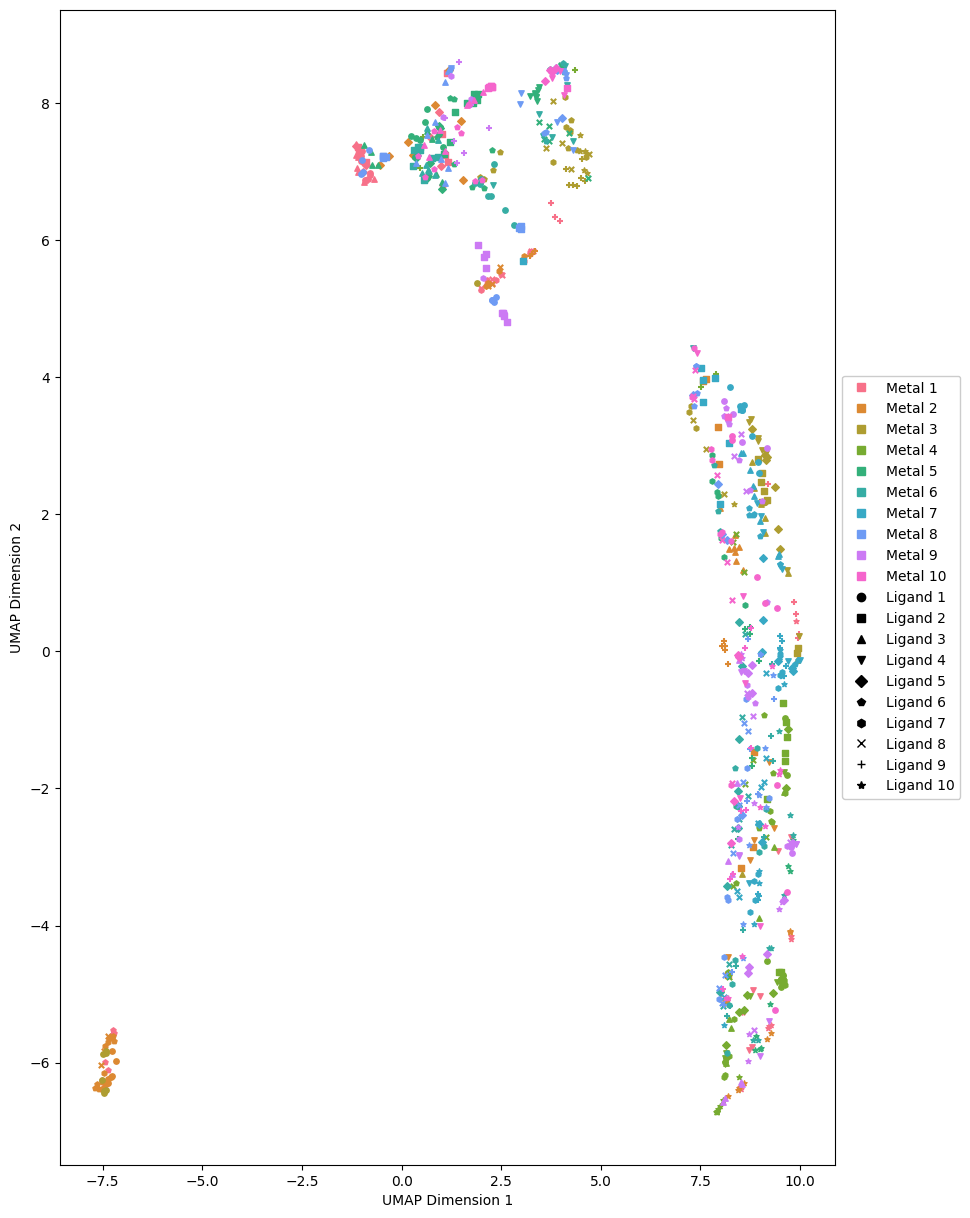
\includegraphics[width=1.0\textwidth]{figures/cv_umap.png}
    \caption{Cyclic Voltammetry UMAP Projection}
    \label{cv-umap}
\end{figure}
\begin{figure}[h!]
  \centering
    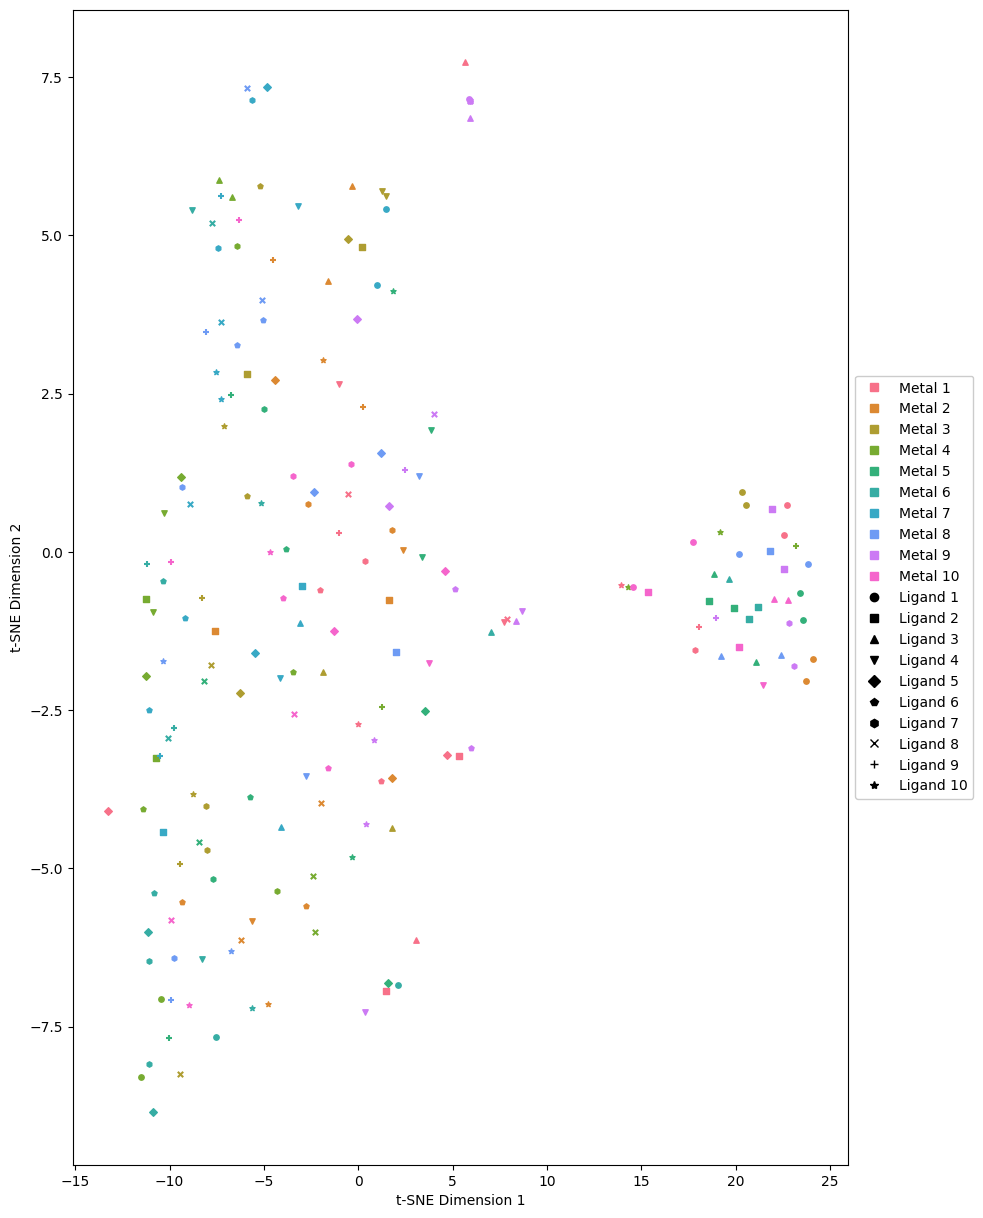
\includegraphics[width=1.0\textwidth]{figures/dpv_tsne.png}
    \caption{Differential Pulse Voltammetry t-SNE Projection}
    \label{dpv-tsne}
\end{figure}
\begin{figure}[h!]
  \centering
    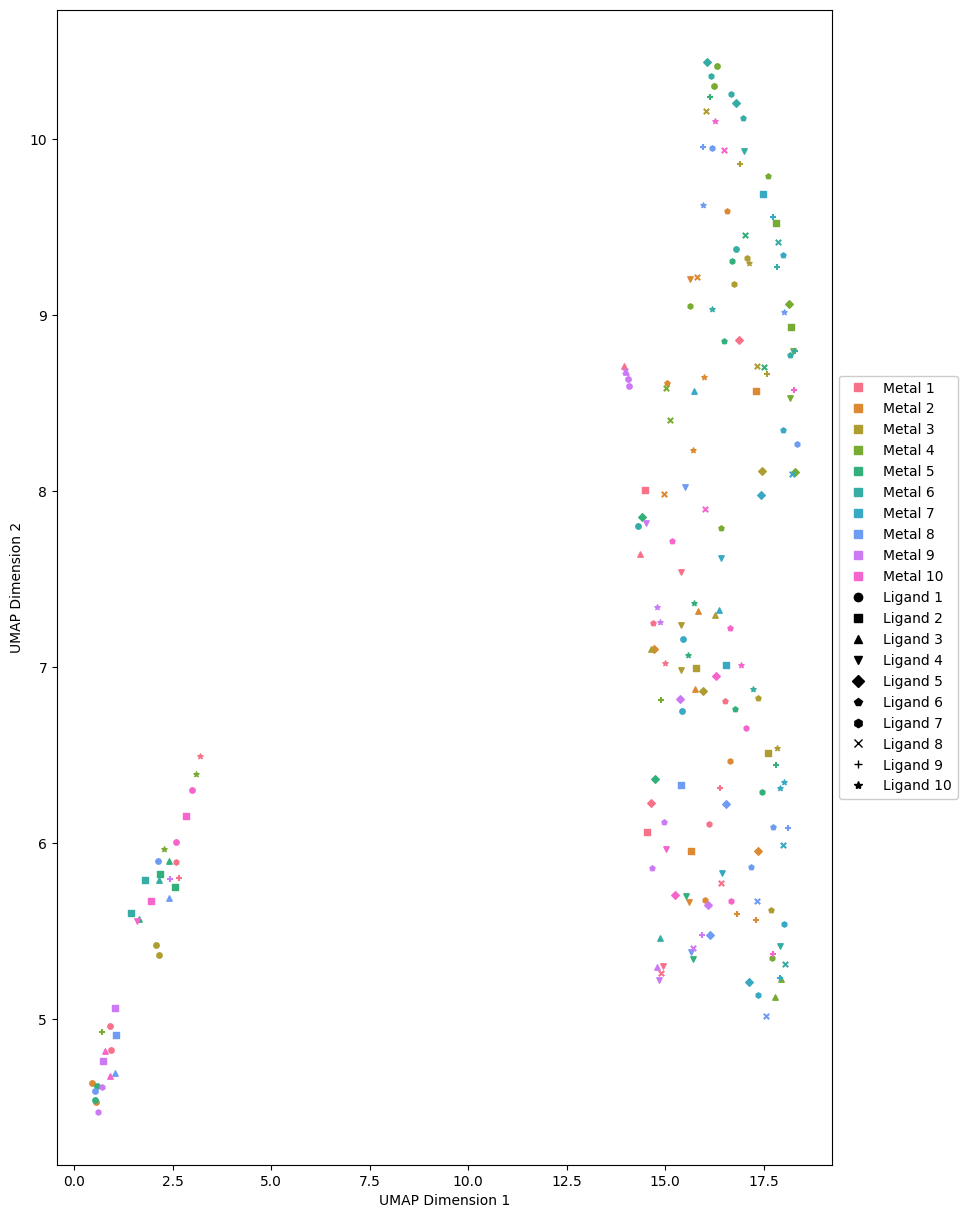
\includegraphics[width=1.0\textwidth]{figures/dpv_umap.png}
    \caption{Differential Pulse Voltammetry UMAP Projection}
    \label{dpv-umap}
\end{figure}
Using machine learning techniques to classify voltammetry data according to the overall shape offers several advantages over simply using a script to find the number of peaks. Machine learning models can be trained to recognize patterns and variations regarding the overall shape and number of peaks. They can adapt to experimental conditions, electrode materials, and analytes without needing manual adjustment of parameters. Voltammetry data can often be noisy, especially at low concentrations. ML models can be trained to distinguish true peaks from noise more effectively than simple peak-finding algorithms. Voltammograms can vary in characteristics due to factors such as electrode deterioration, surface roughness, and solution composition. ML models can learn to handle this variability and provide more reliable peak classification across different experimental conditions. Additionally, ML models can learn when the electrode deteriorates and automatically polish it. ML models can automatically extract relevant features from voltammogram data such as peak heights, peak widths, peak potential, and overall shape. This allows for more comprehensive analysis beyond locating peaks. Once trained, ML models can be integrated into larger data analysis pipelines to classify cyclic voltammetry data rapidly and efficiently, potentially saving time and effort compared to manual analysis or parameter tuning for peak-finding algorithms.  